%%%%%%%%%%%%%%%%% PREAMBLE %%%%%%%%%%%%%%%%%%%%%%%%%%%%
%Change the font size of your document - 10pt, 12.1pt, etc.
\documentclass[letterpaper,12pt,oneside]{article}
\usepackage[utf8]{inputenc}
\usepackage[T1]{fontenc}
\usepackage[british]{babel}
\usepackage{setspace}
\usepackage{hyperref}
\usepackage{xurl}
\usepackage{graphicx}
\usepackage{array}
\usepackage[left=1.02in, right=1.02in, bottom=1.15in, top=0.85in]{geometry}
\usepackage[pages=all]{background}
\usepackage{transparent}

\hypersetup{colorlinks=true, urlcolor=blue, linkcolor=black}

% Suppress printed page numbers while retaining unique internal page identifiers.
\pagestyle{empty}

%%%%%%%%%%%%%%%%% COURSE PARAMETERS %%%%%%%%%%%%%%%%%%%
% These two values are yours to set once enrolment is known.
% They propagate to every place in the document where the value is mentioned.

\newcommand{\maxgroupsize}{3}          % max students per group (not fixed by FS)
\newcommand{\numprojects}{3--6}        % must stay within the 3-6 range fixed by FS

% NOT parameterised on purpose - these are fixed by the FS course description
% and cannot be changed for this run of the course:
%   portfolio = GROUP projects, weight 1/2, collective grade
%   exam      = INDIVIDUAL oral, 30 min, weight 1/2, no aids
%   both parts must be passed; no resit opportunities

%%%%%%%%%%%%%%%%% END OF PREAMBLE %%%%%%%%%%%%%%%%%%%%%

\backgroundsetup{
scale=1,
color=black,
opacity=0.16,
angle=0,
contents={%
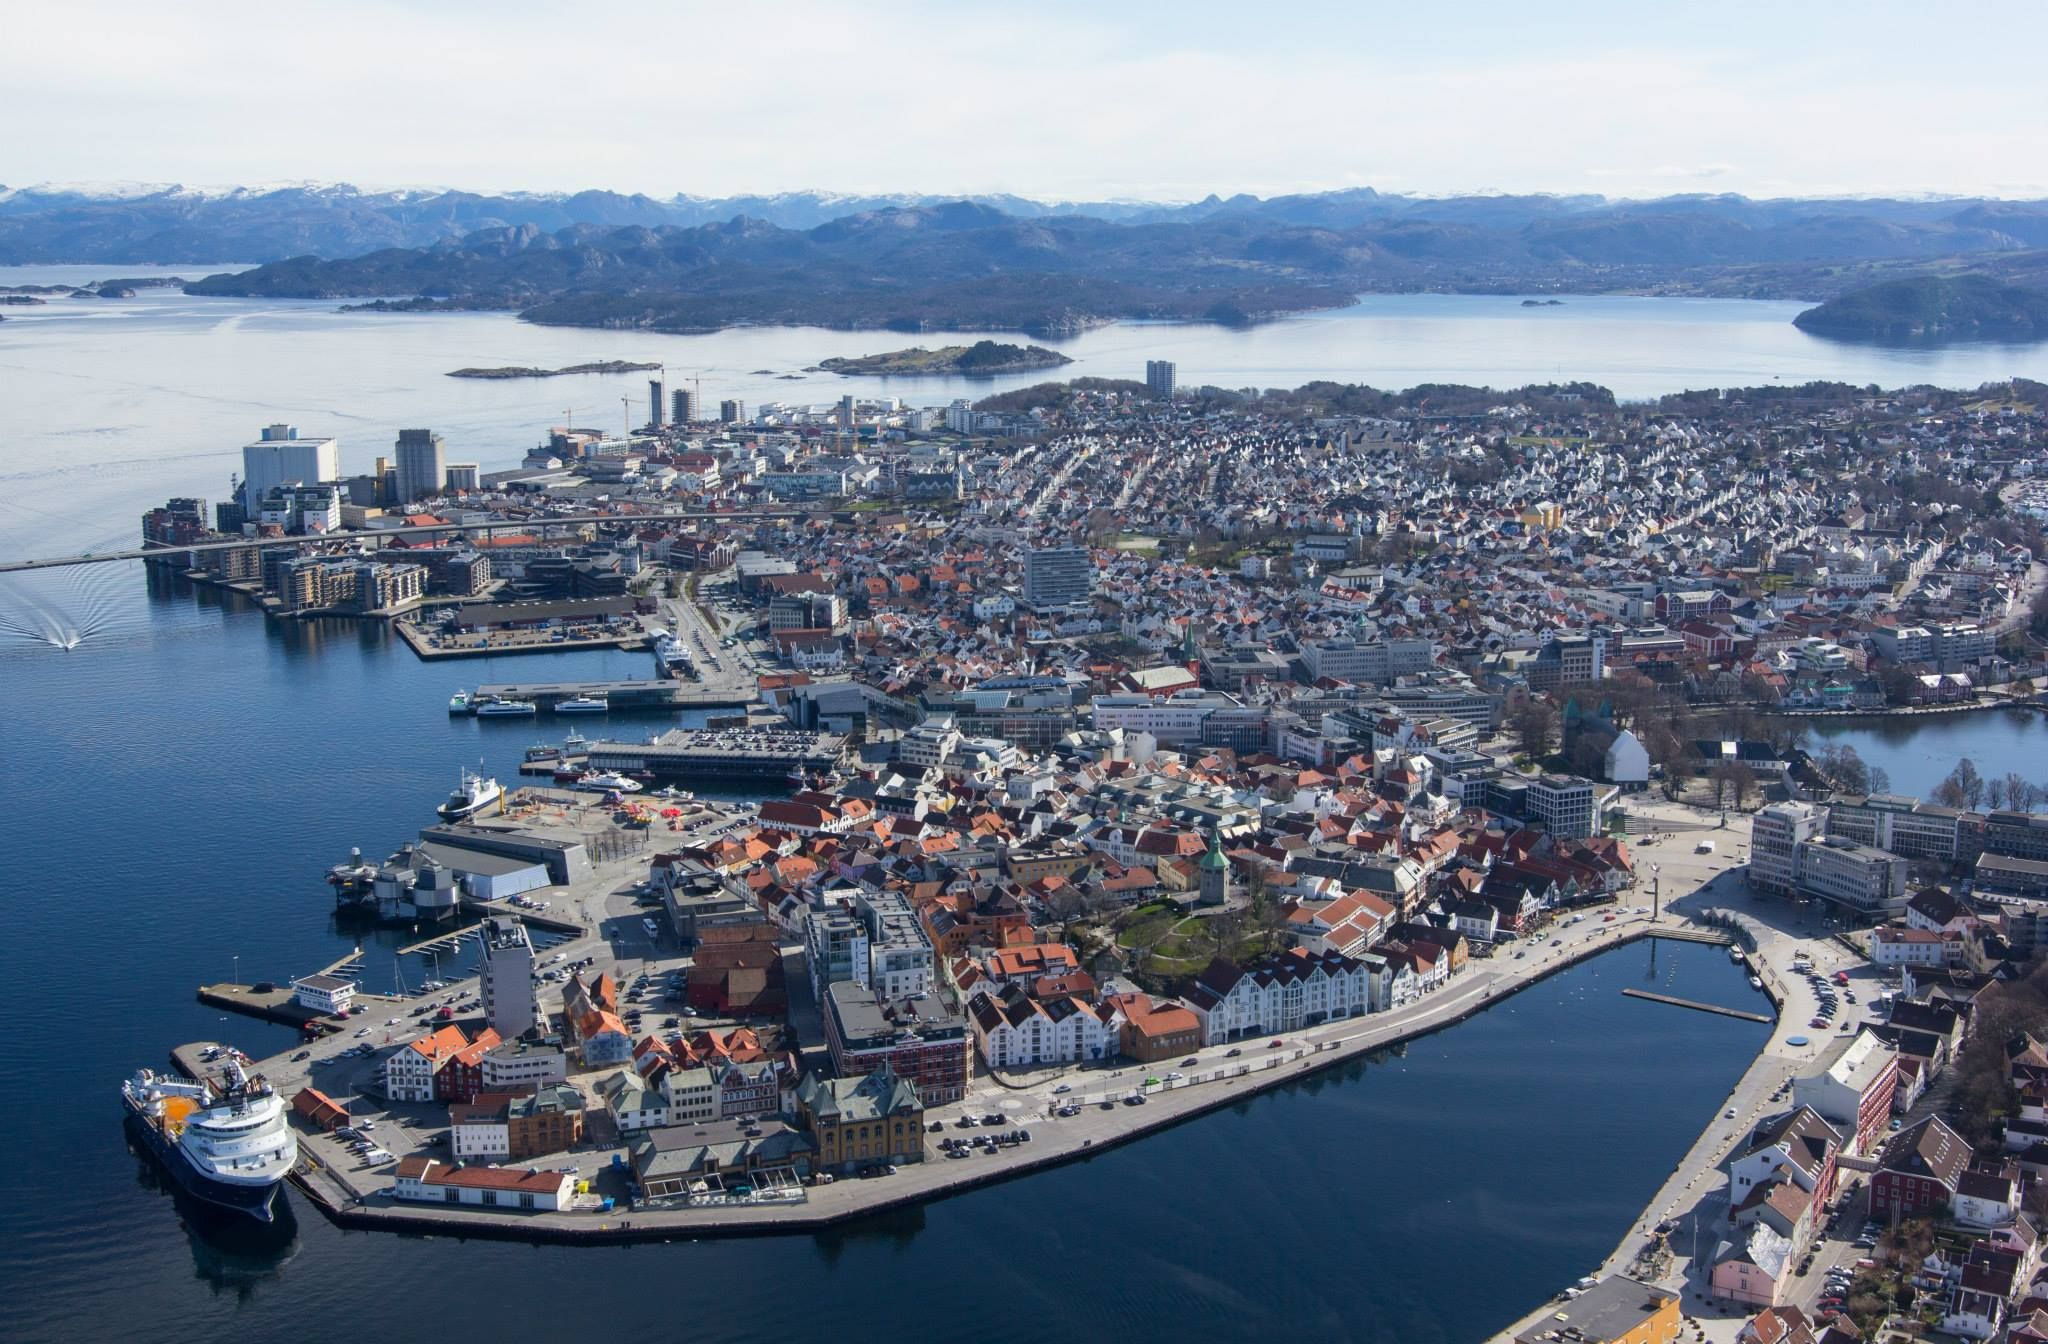
\includegraphics[width=\paperwidth,height=\paperheight]{stv.jpg}
}%
}
\begin{document}
\begin{flushright}
\transparent{0.99}
\includegraphics[scale=0.5]{uis_logo.jpeg}
\end{flushright}


\vspace{-8.3em}
\begin{flushleft}
\Large\textit{\bfseries --- Course Overview ------------------- \\
MOD550: Fundaments of Machine \\ Learning for and with \\
Engineering Applications \\ Autumn 2026 \\ }
\end{flushleft}

---------------------------------------------------------------------------------------

\vspace{1.5em}

\begin{flushleft}
\textit{``The goal is to turn data into information, and information into insight''} \\
Carly Fiorina, Former CEO of HP

\end{flushleft}

\section*{Facts}

\begin{tabbing}
\hspace{13em}\= \kill
Course code \> MOD550 \\
Credits (ECTS) \> 10 \\
Semester tuition start \> Autumn \\
Number of semesters \> 1 \\
Exam semester \> Spring, Autumn \\
Language of instruction \> English \\
Offered by \> Faculty of Science and Technology, \\
 \> Department of Mathematics and Physics \\
\end{tabbing}

\section*{Introduction}
Machine learning provides engineers with tools for building predictive models, quantifying uncertainty, optimising systems, and supporting decisions with data. In this course, students apply statistical and machine-learning methods to engineering problems in fields such as mechanical and chemical engineering, geoscience, and materials science. The emphasis is on combining physical understanding with data-driven modelling to address real-world problems.

Students enter the course with different strengths in engineering, programming, mathematics, and statistics. The course provides a common entry point and helps connect these perspectives.

\section*{Learning outcomes}

\subsection*{Knowledge}
\begin{itemize}
\item Understanding of engineering data sources and consequent data properties, statistics, and probability distributions (from feature engineering to digital twins).
\item Understanding of data analysis/machine learning approaches outcomes, method sensitivity and their applications (e.g.\ molecular modelling, flow simulation, geoscience).
\item Understanding of deep learning principles and its advantages/limitations in engineering applications.
\item Ability to construct basic predictive models (e.g.\ Monte Carlo simulations, language models such as ChatGPT).
\end{itemize}

\subsection*{Skills}
\begin{itemize}
\item Data handling, data wrangling and feature engineering.
\item Can develop data-driven models of physical systems for chemical and mechanical engineering, materials science and geology.
\item Test data-driven models against physical models and experimental data.
\item Apply appropriate statistical methods to obtain better insights.
\item Develop own programs written in Python and develop wrappers for open machine learning repositories.
\end{itemize}

\subsection*{General competence}
\begin{itemize}
\item Can identify engineering problems, develop hypotheses, and apply mathematical models and data-driven solutions.
\item Can structure different statistical models in a wide range of engineering applications.
\item Can connect engineers and data science solutions -- both to specialists and to the general public.
\end{itemize}


\section*{Content}


The course focuses on statistical and machine-learning methods for spatial and temporal engineering data, with particular attention to the assumptions that make those methods appropriate. Students examine how data sources, quality, and consistency affect model selection and interpretation.

Simulation techniques are used to represent heterogeneity and uncertainty. Methods include regression, multivariate data analysis, and predictive machine learning. Python and related tools are used to prepare data, build and evaluate models, automate statistical workflows, and create visualisations that communicate the results.

The purpose of modelling is to provide decision-relevant insight. In each task, models will therefore be evaluated in terms of interpretability, appropriate resolution, predictive accuracy, and usefulness for the decision at hand.

Topics covered during the semester include, among others:

\begin{itemize}
\item Multivariate data analysis, including principal component, cluster, and discriminant analysis.
\item Machine learning techniques for predictive modelling (e.g.\ random forest, gradient boosting machine, support vector regression, and kriging models).
\item Sensitivity analysis and the information it provides.
\item Visualisation and reporting, to provide input for a decision by communicating information to decision-makers.
\end{itemize}


\section*{Course Staff}

Course coordinator and teacher:

Enrico Riccardi

Email: enrico.riccardi@uis.no

Office: KE E-542

\vspace{1em}

Course teacher:

Auref Rostamian

Email: auref.rostamian@uis.no


\section*{Class Delivery}

We will meet physically in the lecture room 6 hours per week most of the semester, as lectures with scheduled tutorials. Students are expected to spend an additional 6--8 hours a week on self-study and assignments.

The course is organised in \textbf{modules}. A module spans several sessions and follows the same three-part progression:

\begin{enumerate}
\item \textbf{Theory.} The concepts, assumptions and methods needed for the task at hand.
\item \textbf{Task identification and discussion.} We frame the problem together, decide what a useful answer looks like, and agree on how it will be evaluated.
\item \textbf{Task completion.} You work on the task, with the instructors available.
\end{enumerate}

Two kinds of work run in parallel, and it is worth keeping them apart:

\begin{itemize}
\item \textbf{Exercises.} Smaller problems worked through during the sessions. They are not graded. We discuss them openly in class, and solutions are shown and made available.
\item \textbf{Assignments (module deliverables).} \textbf{Each module closes with a deliverable}, in which your group applies what the module covered. These are the graded work: together they form the portfolio.
\end{itemize}

Assignments are also discussed in class, but \textbf{within limits set by the size of the group}: we cannot go through every delivery individually, so feedback on the assignments is given at the level of common patterns, recurring mistakes and the range of approaches taken, rather than as a full review of each submission. Model solutions to the assignments are not published, since they are the assessed work.

A great deal of the learning and value of this course comes from in-class discussions; therefore, attending lectures regularly and keeping up with the readings and assignments is essential to ensure a rewarding learning experience (as well as a good grade). The lectures will include some interactive computer work (not recorded). Independent readings throughout the semester are expected and attendance is not mandatory (but strongly recommended).

\textbf{Remote participation may be arranged on request.} The course is designed for on-site delivery, and the discussion and task work are where most of the learning takes place. Where circumstances prevent a student from being present -- for instance reduced mobility, illness, or other documented grounds -- a remote connection to the session may be arranged. Such requests must be directed to the instructors \textbf{in advance of the session concerned}, as the arrangement cannot be made retrospectively.

The sessions will also include interactive Python implementations and coding. You are expected to have Python installed (more information on Canvas) on your computers. The interactive sessions will expand upon and add details to the curriculum covered in the lectures. In these sessions we will show examples of how to use and implement models and analyses discussed, illustrate how to solve problems, work through exercises and respond to any questions you may have on the curriculum. Jupyter Notebooks and exercise solutions will be made available on Canvas.

\section*{Group Work}

The portfolio is carried out in groups of \textbf{at most \maxgroupsize{} students}. This is a ceiling, not a target: there is no minimum group size, so a group of two -- or working on your own -- is equally acceptable. Groups organise their own work, but every member is expected to contribute to, and be able to explain, every part of a delivery.

The number of portfolio projects is \textbf{confirmed at the start of the semester}.

The group receives a collective grade on the portfolio. \textbf{The oral exam is individual}: it is where each of you demonstrates that the work submitted under your name is genuinely yours.

\section*{Use of AI}

Generative AI is a tool of this course, not a violation of it. \textbf{You are expected to use AI, and its use is supported and encouraged} -- as an assistant for coding, exploration, and writing.

Two conditions apply:

\begin{itemize}
\item \textbf{You remain responsible for what you deliver.} The submission is yours: its correctness, its choices, and its claims. ``The model wrote it'' is not a defence for an error you handed in.
\item \textbf{You must be able to do, and to account for, the work.} The oral exam is passed only if you demonstrate that \emph{you} did the work -- that you understand the methods used, why they were chosen, and what the results mean. A delivery you cannot explain will not earn a pass, however good it looks.
\end{itemize}

A statement on AI usage has to be included \textbf{in each assignment}, describing which tools were used and for what.

\section*{First day of lectures}

Wednesday 19 August 2026


\section*{Schedule and location}

The up-to-date timetable, including rooms, is available from the \href{https://tp.educloud.no/uis/timeplan/timeplan.php?id=MOD550&type=course&hide_old=1}{UiS timetable for MOD550}.


\section*{Recommended background}

There is no formal prerequisite for this course. That said, the course assumes a BSc in Engineering/Economics/Mathematics/Geoscience, and a basic understanding of coding.

The course is open to students admitted to Computational Engineering (Master), Energy, Reservoir and Earth Sciences (Master), Industrial Asset Management (Master), exchange programmes at the Faculty of Science and Technology, and single courses at Master level at the Faculty.


\section*{Assessment}

The grade for the course is based on two parts, each weighted one half:

\vspace{0.5em}
\begin{center}
\begin{tabular}{|l|c|l|l|l|}
\hline
\textbf{Part} & \textbf{Weight} & \textbf{Duration} & \textbf{Marks} & \textbf{Aids} \\
\hline
Portfolio & 1/2 & Semester & Letter grades & All \\
\hline
Oral exam & 1/2 & 30 minutes & Letter grades & None permitted \\
\hline
\end{tabular}
\end{center}
\vspace{0.5em}

The portfolio consists of \numprojects{} different group projects -- one per module, delivered as each module closes -- to which a collective grade is given when all parts are submitted and assessed. The exact number of projects, and the group composition, will be announced at the start of the semester.

\textbf{The oral exam is a discussion of your projects.} It is individual, lasts 30 minutes, and takes your portfolio deliveries as its starting point: expect to explain what your group did, why those choices were made, and what the results mean. Questions may extend from your projects to the course material they build on.

\textbf{Deadlines.} Each module deliverable has a submission deadline, announced on Canvas. \textbf{Any delay must be agreed in advance} with the instructors. Penalties will be applied to late deliveries that have not been agreed beforehand.

\textbf{Both the portfolio and the oral exam must be passed} to receive a passing grade in the course.

% PENDING (asked 2026-08-18): can a single additional ORAL sitting be offered as a
% resit? FS 2026-27 currently states "no resit opportunities", so the paragraph below
% must stay as-is until the exam office / department confirms otherwise.
% If confirmed -> replace this paragraph with the one-more-oral-attempt wording.
\textbf{There are no resit opportunities} for the assessments. Students who do not pass, or who wish to improve their grade, must retake all the assessment parts the next time the course is offered -- including the parts already passed.

Students may discuss the assignments across groups, but each delivery must be the work of the group that hands it in, and must not be a copy of another's.


\section*{Modelling and Programming}

Many of the assignments will require the development of models and solving them by programming in Python. We will provide Python tutorials on Canvas and show live coding during interactive sessions. However, you should also actively integrate your Python fluency with the web platforms and AI tools available to you.


\section*{Literature}

\textbf{No textbook is compulsory.} The lectures are self-contained, and the material needed for the assignments is covered in class and on Canvas. The following are recommended for the independent reading expected during the semester; the first three are freely available online, legally, from the authors.

\subsection*{Books}

\begin{itemize}
\item S.~L. Brunton and J.~N. Kutz, \textit{Data-Driven Science and Engineering: Machine Learning, Dynamical Systems, and Control}, 2nd ed., Cambridge University Press, 2022. \\ The closest match to this course: machine learning framed for engineers and physical systems. Free PDF: \href{https://databookuw.com/}{databookuw.com}
\item G.~James, D.~Witten, T.~Hastie, R.~Tibshirani and J.~Taylor, \textit{An Introduction to Statistical Learning, with Applications in Python}, Springer, 2023. \\ The best entry point to the statistical side, at the right level, with Python labs. Free PDF: \href{https://www.statlearning.com/}{statlearning.com}
\item T.~Hastie, R.~Tibshirani and J.~Friedman, \textit{The Elements of Statistical Learning}, 2nd ed., Springer, 2009. \\ The reference to consult when you want the theory behind a method. Free PDF: \href{https://hastie.su.domains/ElemStatLearn/}{hastie.su.domains/ElemStatLearn}
\item A.~G\'eron, \textit{Hands-On Machine Learning with Scikit-Learn, Keras and TensorFlow}, 3rd ed., O'Reilly, 2022. \\ The most practical of the four, if you prefer to learn by building.
\end{itemize}

\subsection*{Online}

\begin{itemize}
\item \textit{scikit-learn user guide} -- the library used throughout the course, and unusually good documentation in its own right: \href{https://scikit-learn.org/stable/user_guide.html}{scikit-learn.org/stable/user\_guide.html}
\item J.~VanderPlas, \textit{Python Data Science Handbook} -- NumPy, pandas and matplotlib, free to read online: \href{https://jakevdp.github.io/PythonDataScienceHandbook/}{jakevdp.github.io/PythonDataScienceHandbook}
\item The UiS reading list for this course is maintained in Leganto, reachable from the course page at \href{https://www.uis.no/en/course/MOD550_1}{uis.no/en/course/MOD550\_1}
\end{itemize}


\section*{Course evaluation}

\textbf{An early dialogue will be held in this course.} The aim is to collect your feedback early enough that it can still change how the rest of the semester runs, rather than only benefiting next year's students.

\textbf{Feedback is encouraged at any point}, not only at the scheduled dialogue. If something is not working -- pace, difficulty, the balance between theory and task work, the assignments -- say so, to either of us, and we will look at it. In addition, a digital course evaluation is conducted at least every three years to gather students' experiences.

\textbf{We strongly encourage you to leave feedback on the course at the end of the semester.} It will be very much taken into consideration, and it helps the course better meet students' priorities. The end-of-semester feedback is the one that shapes what this course becomes: it is read carefully, and it is the main reason the course changes from one year to the next.


\vspace{3em}
\section*{Looking forward to meeting you}

\end{document}
